\documentclass[tikz]{standalone}

\usepackage{stix2}

\usetikzlibrary{cd}
\usetikzlibrary{calc}
\tikzcdset{arrow style=math font}

% https://tex.stackexchange.com/a/159141
\pgfdeclarelayer{background}
\pgfdeclarelayer{foreground}
\pgfsetlayers{background,main,foreground}

\begin{document}
  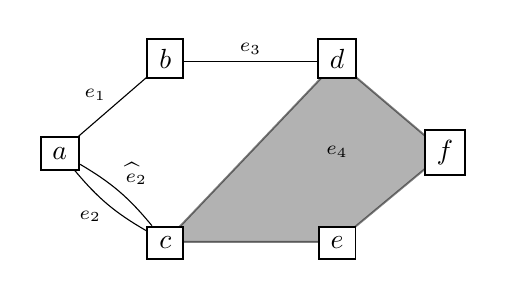
\begin{tikzpicture}[commutative diagrams/every diagram]
    \matrix
      [
        matrix of math nodes,
        name=m,
        commutative diagrams/every cell,
        cells={nodes={draw=black, fill=white, line width=0.25mm}}
      ]
      {
          & b && d & \\
        a &   &&   & f \\
          & c && e & \\
      };
    \path[commutative diagrams/.cd, every arrow, dash, every label]
      (m-2-1) edge["$e_1$"] (m-1-2)
      (m-2-1) edge[swap, bend right=10, "$e_2$"] (m-3-2)
      (m-2-1) edge["$\widehat e_2$", bend left=10] (m-3-2)
      (m-1-2) edge["$e_3$"] (m-1-4);
    \node[commutative diagrams/.cd, every label] at ($(m-1-4.center)!0.5!(m-3-4.center)$) {$e_4$};
    \begin{pgfonlayer}{background}
      \fill[commutative diagrams/.cd, draw=black, opacity=0.5, fill=black, fill opacity=0.3, line width=0.25mm]
          (m-3-2.center) -- (m-3-4.center) -- (m-2-5.center) -- (m-1-4.center) -- cycle;
    \end{pgfonlayer}
  \end{tikzpicture}
\end{document}
